% Netherite mid submission. Based on the official ACL LuaLaTeX/XeLaTeX template (acl_lualatex.tex).
% Compile with LuaLaTeX or XeLaTeX (the text contains Devanagari), not pdfLaTeX.
\documentclass[11pt]{article}

\usepackage[final]{acl}

\usepackage{microtype}
\usepackage[english,bidi=default]{babel}
\babelfont{rm}{TeXGyreTermesX}
\babelprovide[import, hyphenrules=nohyphenation]{hindi}
\IfFontExistsTF{Lohit Devanagari}
  {\babelfont[*devanagari]{rm}{Lohit Devanagari}}
  {\babelfont[*devanagari]{rm}{Kohinoor Devanagari}}

\usepackage{amsmath}
\usepackage{amssymb}
\usepackage{graphicx}
\usepackage{booktabs}
\usepackage{tikz}
\usetikzlibrary{arrows.meta,positioning,calc}
\newcommand{\AEnCotShort}{99.3}
\newcommand{\AEnCotVeryLong}{97.3}
\newcommand{\AEnDirectShort}{97.0}
\newcommand{\AEnDirectVeryLong}{81.1}
\newcommand{\AHiCotShort}{92.8}
\newcommand{\AHiCotVeryLong}{78.8}
\newcommand{\AHiDirectShort}{94.0}
\newcommand{\AHiDirectVeryLong}{74.0}
\newcommand{\AgreeCotBothRight}{5,565}
\newcommand{\AgreeCotBothWrong}{609}
\newcommand{\AgreeCotEnOnly}{2,585}
\newcommand{\AgreeCotHiOnly}{172}
\newcommand{\AgreeCotPairs}{8,931}
\newcommand{\AgreeCotPhi}{0.05}
\newcommand{\AgreeDirectBothRight}{4,729}
\newcommand{\AgreeDirectBothWrong}{2,785}
\newcommand{\AgreeDirectEnOnly}{1,115}
\newcommand{\AgreeDirectHiOnly}{622}
\newcommand{\AgreeDirectPairs}{9,251}
\newcommand{\AgreeDirectPhi}{0.31}
\newcommand{\CoveragePct}{46}
\newcommand{\DriftDow}{181}
\newcommand{\DriftDowAcc}{34.3}
\newcommand{\DriftDowAccNo}{19.8}
\newcommand{\DriftOR}{1.94}
\newcommand{\DriftORHi}{2.64}
\newcommand{\DriftORLo}{1.43}
\newcommand{\DriftP}{\(p<0.001\)}
\newcommand{\DriftRec}{37}
\newcommand{\DriftRecAcc}{51.4}
\newcommand{\DriftRecAccNo}{25.3}
\newcommand{\DriftStrata}{12}
\newcommand{\EnAnswerInTrace}{99.9}
\newcommand{\EnCotAcc}{91.1}
\newcommand{\EnCotDelta}{+27.9}
\newcommand{\EnCotDeltaHi}{+29.3}
\newcommand{\EnCotDeltaLo}{+26.6}
\newcommand{\EnCotWins}{2,603}
\newcommand{\EnDidDis}{$-$0.8}
\newcommand{\EnDidDisHi}{+0.9}
\newcommand{\EnDidDisLo}{$-$2.7}
\newcommand{\EnDidSim}{+0.0}
\newcommand{\EnDidSimHi}{+1.8}
\newcommand{\EnDidSimLo}{$-$1.7}
\newcommand{\EnDirectAcc}{63.2}
\newcommand{\EnDirectWins}{204}
\newcommand{\EnDowCot}{70.5}
\newcommand{\EnDowCotMinusOne}{6.2}
\newcommand{\EnDowCotPlusOne}{17.4}
\newcommand{\EnDowDelta}{+56.4}
\newcommand{\EnDowDirect}{14.1}
\newcommand{\EnDowDirectMax}{15.1}
\newcommand{\EnDowDirectMin}{12.7}
\newcommand{\EnDowModeDay}{Friday}
\newcommand{\EnDowModeShare}{35.4}
\newcommand{\EnDropCotDis}{+0.4}
\newcommand{\EnDropCotSim}{+0.9}
\newcommand{\EnDropDirectDis}{+1.2}
\newcommand{\EnDropDirectSim}{+0.9}
\newcommand{\EnErrAddMonthSlip}{0.0}
\newcommand{\EnErrAddOffByOne}{88.9}
\newcommand{\EnErrAllN}{798}
\newcommand{\EnErrAllOffByOne}{66.5}
\newcommand{\EnErrDowMonthSlip}{0.0}
\newcommand{\EnErrDowOffByOne}{79.8}
\newcommand{\EnErrSubMonthSlip}{0.0}
\newcommand{\EnErrSubOffByOne}{85.5}
\newcommand{\EnIntervalCot}{43.1}
\newcommand{\EnIntervalDelta}{+13.3}
\newcommand{\EnIntervalDirect}{29.8}
\newcommand{\EnMaxDrop}{1.2}
\newcommand{\EnMedianTokens}{327}
\newcommand{\EnMedianWords}{103}
\newcommand{\EnMentionDis}{18.7}
\newcommand{\EnMentionDisOR}{1.33}
\newcommand{\EnMentionDisORHi}{2.15}
\newcommand{\EnMentionDisORLo}{0.82}
\newcommand{\EnMentionDisOddsDrop}{-33}
\newcommand{\EnMentionDisP}{\(p=0.25\)}
\newcommand{\EnMentionDisPlacebo}{8.5}
\newcommand{\EnMentionSim}{15.1}
\newcommand{\EnMentionSimOR}{0.64}
\newcommand{\EnMentionSimORHi}{0.93}
\newcommand{\EnMentionSimORLo}{0.44}
\newcommand{\EnMentionSimOddsDrop}{36}
\newcommand{\EnMentionSimP}{\(p=0.02\)}
\newcommand{\EnMentionSimPlacebo}{10.4}
\newcommand{\EnRatioBelow}{0.0}
\newcommand{\EnRatioPooled}{1.000}
\newcommand{\EnRecCotFirstStep}{0.1}
\newcommand{\EnRecCotMirror}{0.5}
\newcommand{\EnRecDirectFirstStep}{31.3}
\newcommand{\EnRecDirectMirror}{1.1}
\newcommand{\EnRecSimDropCot}{+6.9}
\newcommand{\EnRecurrenceCot}{92.4}
\newcommand{\EnRecurrenceDelta}{+67.9}
\newcommand{\EnRecurrenceDirect}{24.5}
\newcommand{\EnReuseCot}{0.0}
\newcommand{\EnReuseCotN}{0 of 127}
\newcommand{\EnReuseCotP}{\(p=0.47\)}
\newcommand{\EnReuseCotPlacebo}{0.9}
\newcommand{\EnReuseCotPlaceboN}{1 of 113}
\newcommand{\EnReuseDirect}{4.9}
\newcommand{\EnReuseDirectN}{25 of 511}
\newcommand{\EnReuseDirectP}{\(p=0.45\)}
\newcommand{\EnReuseDirectPlacebo}{3.9}
\newcommand{\EnReuseDirectPlaceboN}{20 of 513}
\newcommand{\EnStrictDelta}{+25.3}
\newcommand{\EnSubtractionCot}{95.9}
\newcommand{\EnSubtractionDelta}{+2.3}
\newcommand{\EnSubtractionDirect}{93.6}
\newcommand{\EnTimeDurationCot}{99.8}
\newcommand{\EnTimeDurationDelta}{+40.9}
\newcommand{\EnTimeDurationDirect}{58.8}
\newcommand{\EnVerification}{79.1}
\newcommand{\EnWrong}{798}
\newcommand{\EnWrongEndsGold}{1}
\newcommand{\GapACotLong}{9.6}
\newcommand{\GapACotShort}{6.6}
\newcommand{\GapACotVeryLong}{18.5}
\newcommand{\GapADirectLong}{3.5}
\newcommand{\GapADirectShort}{3.0}
\newcommand{\GapADirectVeryLong}{7.1}
\newcommand{\GapCotShort}{27.0}
\newcommand{\GapCotVeryLong}{40.4}
\newcommand{\GapDirectShort}{8.6}
\newcommand{\GapDirectVeryLong}{6.6}
\newcommand{\HiAccRatioAbove}{63.5}
\newcommand{\HiAccRatioBelow}{37.5}
\newcommand{\HiAnswerInTrace}{99.0}
\newcommand{\HiCotAcc}{62.9}
\newcommand{\HiCotDelta}{+5.1}
\newcommand{\HiCotDeltaHi}{+6.4}
\newcommand{\HiCotDeltaLo}{+3.8}
\newcommand{\HiCotWins}{1,458}
\newcommand{\HiDidDis}{+2.8}
\newcommand{\HiDidDisHi}{+4.9}
\newcommand{\HiDidDisLo}{+0.7}
\newcommand{\HiDidSim}{+5.2}
\newcommand{\HiDidSimAbs}{5.2}
\newcommand{\HiDidSimDow}{+8.0}
\newcommand{\HiDidSimDowHi}{+14.2}
\newcommand{\HiDidSimDowLo}{+1.3}
\newcommand{\HiDidSimDuration}{+10.3}
\newcommand{\HiDidSimDurationHi}{+15.1}
\newcommand{\HiDidSimDurationLo}{+5.3}
\newcommand{\HiDidSimHi}{+7.3}
\newcommand{\HiDidSimLo}{+2.9}
\newcommand{\HiDidSimRec}{+5.8}
\newcommand{\HiDidSimRecHi}{+11.5}
\newcommand{\HiDidSimRecLo}{$-$0.0}
\newcommand{\HiDidSimTimeDuration}{+22.1}
\newcommand{\HiDidSimTimeDurationHi}{+35.5}
\newcommand{\HiDidSimTimeDurationLo}{+8.3}
\newcommand{\HiDirectAcc}{57.7}
\newcommand{\HiDirectWins}{1,012}
\newcommand{\HiDowCot}{21.8}
\newcommand{\HiDowCotPlusOne}{25.7}
\newcommand{\HiDowCotZero}{21.8}
\newcommand{\HiDowDelta}{+6.1}
\newcommand{\HiDowDirect}{15.7}
\newcommand{\HiDowDirectMax}{15.7}
\newcommand{\HiDowDirectMin}{12.7}
\newcommand{\HiDowModeDay}{Sunday}
\newcommand{\HiDowModeShare}{63.4}
\newcommand{\HiDropCotDis}{+2.5}
\newcommand{\HiDropCotSim}{+4.5}
\newcommand{\HiDropCotSimAbs}{4.5}
\newcommand{\HiDropDirectDis}{$-$0.3}
\newcommand{\HiDropDirectSim}{$-$0.7}
\newcommand{\HiErrAddMonthSlip}{17.5}
\newcommand{\HiErrAddOffByOne}{34.1}
\newcommand{\HiErrAllN}{3,416}
\newcommand{\HiErrAllOffByOne}{27.1}
\newcommand{\HiErrDowMonthSlip}{0.0}
\newcommand{\HiErrDowOffByOne}{45.4}
\newcommand{\HiErrSubMonthSlip}{4.4}
\newcommand{\HiErrSubOffByOne}{22.9}
\newcommand{\HiIntervalCot}{17.9}
\newcommand{\HiIntervalDelta}{$-$17.2}
\newcommand{\HiIntervalDirect}{35.1}
\newcommand{\HiMedianTokens}{198}
\newcommand{\HiMedianWords}{79}
\newcommand{\HiMentionDis}{35.9}
\newcommand{\HiMentionDisOR}{1.11}
\newcommand{\HiMentionDisORHi}{1.36}
\newcommand{\HiMentionDisORLo}{0.90}
\newcommand{\HiMentionDisOddsDrop}{-11}
\newcommand{\HiMentionDisP}{\(p=0.35\)}
\newcommand{\HiMentionDisPlacebo}{1.4}
\newcommand{\HiMentionSim}{31.8}
\newcommand{\HiMentionSimOR}{0.77}
\newcommand{\HiMentionSimORHi}{0.95}
\newcommand{\HiMentionSimORLo}{0.63}
\newcommand{\HiMentionSimOddsDrop}{23}
\newcommand{\HiMentionSimP}{\(p=0.01\)}
\newcommand{\HiMentionSimPlacebo}{8.3}
\newcommand{\HiNRatioBelow}{224}
\newcommand{\HiRatioBelow}{2.4}
\newcommand{\HiRatioPooled}{0.986}
\newcommand{\HiRecCotFirstStep}{16.6}
\newcommand{\HiRecCotMirror}{11.8}
\newcommand{\HiRecDirectFirstStep}{31.3}
\newcommand{\HiRecDirectMirror}{10.8}
\newcommand{\HiRecSimDropCot}{+4.7}
\newcommand{\HiRecSimDropDirect}{$-$1.1}
\newcommand{\HiRecurrenceCot}{26.0}
\newcommand{\HiRecurrenceDelta}{+21.2}
\newcommand{\HiRecurrenceDirect}{4.8}
\newcommand{\HiReuseCot}{4.8}
\newcommand{\HiReuseCotN}{29 of 608}
\newcommand{\HiReuseCotP}{\(p=0.04\)}
\newcommand{\HiReuseCotPlacebo}{2.5}
\newcommand{\HiReuseCotPlaceboN}{14 of 559}
\newcommand{\HiReuseDirect}{12.1}
\newcommand{\HiReuseDirectN}{76 of 629}
\newcommand{\HiReuseDirectP}{\(p<0.001\)}
\newcommand{\HiReuseDirectPlacebo}{2.6}
\newcommand{\HiReuseDirectPlaceboN}{16 of 607}
\newcommand{\HiStrictDelta}{+4.7}
\newcommand{\HiSubtractionCot}{78.2}
\newcommand{\HiSubtractionDelta}{$-$14.0}
\newcommand{\HiSubtractionDirect}{92.2}
\newcommand{\HiTimeDurationCot}{72.6}
\newcommand{\HiTimeDurationDelta}{+43.8}
\newcommand{\HiTimeDurationDirect}{28.9}
\newcommand{\HiVerification}{1.5}
\newcommand{\HiWrong}{3,416}
\newcommand{\HiWrongEndsGold}{6}
\newcommand{\NCutoff}{364}
\newcommand{\NCutoffEnCot}{280}
\newcommand{\NCutoffHiCot}{68}
\newcommand{\NCutoffPct}{1.0}
\newcommand{\NEnSigPos}{9}
\newcommand{\NHiSigPos}{5}
\newcommand{\NInvalid}{61}
\newcommand{\NInvalidDirect}{53}
\newcommand{\NPlannedQuestions}{6,750}
\newcommand{\NQuestions}{3,089}
\newcommand{\NRecords}{37,068}
\newcommand{\NScored}{36,704}
\newcommand{\VerAccWith}{89.5}
\newcommand{\VerAccWithout}{97.4}
\newcommand{\VerDowN}{1,117}
\newcommand{\VerDowTotal}{1,141}
\newcommand{\VerOR}{1.33}
\newcommand{\VerORHi}{1.95}
\newcommand{\VerORLo}{0.90}
\newcommand{\VerP}{\(p=0.13\)}


\title{Evaluating Multilingual Reasoning through a Chain-of-Thought Lens}

\author{
  Aayush Batra \quad Aditya Sai \quad Rahul Kannan \quad Shaurya Kochar \\[0.4em]
  Team Netherite \\
  International Institute of Information Technology, Hyderabad, India
}
\begin{document}
\maketitle

\begin{abstract}
Does asking a large language model to think step by step help it reason about time, and does the answer change across languages? We study this with Sarvam-105B on the Temporal Reasoning Dataset (TRD), comparing direct answers with chain-of-thought (CoT) prompting in English and Hindi, with and without controlled distractor sentences. On 3,089 questions answered in all twelve conditions, CoT raises English accuracy by 27.9 percentage points but Hindi accuracy by only 5.1, and it significantly lowers Hindi accuracy on two tasks. The English-Hindi gap under CoT widens with difficulty, and distractors make CoT more fragile only in Hindi, whose reasoning traces often weave the distractor into the solution. Hindi traces stay in Hindi, are shorter, rarely check their work, and fail on different questions from English traces. We describe the problem, related work, our pipeline, the progress so far, and a timeline for the remaining conditions: Hinglish reasoning, cross-lingual prompting, and a structural comparison of English and Hindi traces.
\end{abstract}

\section{Introduction}
\label{sec:intro}

Chain-of-thought (CoT) prompting asks a large language model (LLM) to write out intermediate steps before giving an answer. Surveys describe CoT as a way to break a difficult problem into smaller pieces, and asking for explicit steps can improve multi-step reasoning \citep{wei-etal-2022-chain,huang-chang-2023-towards}. We use ``reasoning trace'' to mean the text the model generates, and we do not assume that this text is a transparent record of its internal computation \citep{turpin-etal-2023-unfaithful}.

The language matters too. The MGSM study found that multilingual models can solve reasoning problems in many languages, but English intermediate steps often perform as well as or better than steps written in the language of the question \citep{shi-etal-2023-mgsm}. That leads to a practical question: if we ask the model to reason in Hindi, does it reason as well as it does in English, and does it get there the same way?

We study this question on temporal reasoning, using the Temporal Reasoning Dataset (TRD) of \citet{mazzia-etal-2026-benchmarking}. TRD generates date and time problems in ten languages at controlled difficulty, and can prepend a distractor sentence to any question. Some distractors relate to time (``I always get confused with months that have 31 days''), while others have nothing to do with the question, such as a sentence about someone buying a motorcycle. This gives us a direct test of our main idea:
\begin{quote}
If a model can ignore the motorcycle when it answers directly, does making it think step by step give the motorcycle more chances to enter its reasoning and derail the answer?
\end{quote}
TRD evaluates its benchmark without CoT, telling the model not to add explanations, and explicitly leaves the effect of CoT on temporal reasoning for future work \citep{mazzia-etal-2026-benchmarking}. We investigate that missing condition, in English and Hindi, with Sarvam-105B \citep{sarvam-2026-models}.

\section{Problem Statement}
\label{sec:problem}

We work with one model, Sarvam-105B, and TRD problems whose answers have a fixed, machine-readable form: a date (YYYY-MM-DD), a clock time (HH:MM), a whole number of days or minutes, a pair of dates for an interval, or a weekday name. Every gold answer has a known form, so responses can be scored automatically.

We vary four things. The question is given in English or Hindi. The distractor is absent, a sentence about time, or a sentence about something unrelated. The prompt is \emph{direct}, which asks only for the answer, or \emph{CoT}, which asks the model to reason step by step; a third prompt, the cross-lingual prompting (CLP) of \citet{qin-etal-2023-cross}, is planned. Whenever we ask for step-by-step reasoning we also choose the language the model should reason in: so far the question's own language, and in the remaining work Hinglish as well. Running the model on one problem gives back the final answer and, in every condition except direct, a reasoning trace.

From the answers we read off differences in accuracy. The \emph{CoT delta} is the change in accuracy when CoT replaces direct answering; a positive delta means step-by-step reasoning helped. The \emph{distraction drop} is how much accuracy falls when a distractor is added. The quantity we care about most combines the two: the \emph{CoT distraction penalty}, the distraction drop under CoT minus the distraction drop under direct answering. If it is positive, thinking out loud gives the distractor room to creep into the answer. We also track the \emph{English--Hindi gap}, English accuracy minus Hindi accuracy, at each difficulty level.

The traces let us look past the final answer. We record how much of a Hindi trace stays in Hindi with the target-language ratio (TLR; Section~\ref{sec:setup}), whether the trace mentions the distractor, and how its final answer relates to its reasoning. In the remaining work we will turn each trace into a short sequence of step types, such as identify a date, add a duration, or check a constraint, and compare the English and Hindi sequences for the same problem. The \emph{reasoning divergence score} (RDS) is the normalised edit distance between the two sequences, so that $0$ means the same structure and $1$ means they share nothing. A logistic regression that predicts whether an answer is wrong from its RDS, difficulty and language will test whether taking a different route goes with more errors.

We ask four questions. (1) Does CoT help, and does that depend on language and difficulty? (2) Does CoT make distractors more harmful, and does that differ by distractor type or language? (3) How does reasoning in Hinglish change accuracy and trace structure? (4) Does CLP beat Hindi CoT and bring Hindi reasoning closer to English? This report answers the first two.

\section{Related Work}
\label{sec:related}

\paragraph{CoT, and when it stops helping.}
\citet{wei-etal-2022-chain} introduced CoT prompting by adding worked examples whose solutions show a chain of natural-language steps; gains appeared mainly in very large models such as PaLM 540B. \citet{kojima2022large} then showed that the examples are not needed: appending ``Let's think step by step'' and running a second prompt to extract the answer raised text-davinci-002 from 17.7\% to 78.7\% on MultiArith and from 10.4\% to 40.7\% on GSM8K. We use this zero-shot form, since TRD has no worked solutions. \citet{wang2023selfconsistency} kept the CoT prompt but sampled several paths and took a majority vote, improving GSM8K by 17.9\%; CLP's ensemble variant reuses that idea. \citet{sprague2025cot} combined a meta-analysis of over 100 papers with their own runs on 20 datasets and 14 models, and found that CoT helps mainly on math and symbolic problems, with most of the benefit coming from executing symbolic steps rather than planning them. \citet{liu2025mind} took six tasks where thinking out loud makes humans worse and showed that models degrade in the same way, with o1-preview losing up to 36.3\% against GPT-4o answering directly. TRD's reasoning tasks are date arithmetic, so the first paper predicts that CoT should help there, while its memorisation tasks look more like recall. Neither lets us assume that CoT always helps.

\paragraph{Distractors and irrelevant context.}
\citet{shi-etal-2023-distracted} built GSM-IC by adding one irrelevant sentence to GSM8K problems, varying its topic, whether it reused a name, and which numbers it carried. Accuracy fell sharply under CoT, zero-shot CoT, least-to-most and program prompting, and self-consistency and an explicit instruction to ignore irrelevant information both helped. \citet{mirzadeh2025gsmsymbolic} turned GSM8K into symbolic templates so that names and numbers could be resampled, and found accuracy moving between versions of the same question and falling as clauses were added; their GSM-NoOp clause, which looks relevant but changes nothing, cost up to 65\%. Neither compares CoT on and off under the same distractor, and both work in English.

\paragraph{Reasoning across languages.}
\citet{shi-etal-2023-mgsm} built MGSM by translating 250 GSM8K problems into ten languages and comparing direct answers, native-language CoT, English CoT and translate-test; English CoT usually matched or beat native CoT. Hindi is not in MGSM, which is one reason we work with TRD. \citet{qin-etal-2023-cross} proposed cross-lingual prompting (CLP): a first stage asks the model to act as an expert in multilingual understanding and to work through the request step by step in a target language, usually English, and a second stage asks it to solve the task from its own restatement. Cross-lingual self-consistent prompting (CLSP) runs the first stage in several languages and votes over the answers. \citet{huang-etal-2023-languages} packed the same idea into one cross-lingual-thought template and narrowed the gap between languages. \citet{lai-nissim-2024-mcot} found that open models do not answer the same math problem consistently across languages and instruction-tuned a 7B model on about 6.3M CoT samples in eleven languages, though Hindi is not among them. For English-centric reasoning models, \citet{yong2025crosslingual} found that more test-time thinking improves multilingual math enough to beat models twice their size, with traces that stay mostly English and quote the non-English input; models reason better in high-resource languages.

\paragraph{Language drift, temporal benchmarks, and trace comparison.}
Models seem to pivot through English internally: Llama-2's middle layers decode more readily to English than to the input language \citep{wendler-etal-2024-llamas}, and \citet{zhao2024handle} describe an understand--solve--respond workflow supported by language-specific neurons. On the output side, \citet{marchisio-etal-2024-understanding} counted how often models answer in the wrong language and found serious confusion in several strong models, and \citet{qi-etal-2025-models} saw the same in reasoning traces: leading models fall back to English, and prompts that force the user's language improve readability but cost accuracy. Our target-language ratio measures whether the model's reasoning stayed in the given language or not. Temporal reasoning has its own benchmarks, including TimeQA, TempReason, MenatQA, TRAM, TimeBench and Test of Time \citep{chen2021timeqa,tan-etal-2023-towards,wei-etal-2023-menatqa,wang-zhao-2024-tram,chu-etal-2024-timebench,fatemi2025test}, but they are English-only and none uses controlled distractors. Code-mixing has benchmarks, including Hindi--English ones \citep{khanuja-etal-2020-gluecos,aguilar-etal-2020-lince,yang-chai-2025-codemixbench}, and code-mixed few-shot examples add to CoT gains \citep{shankar-etal-2024-context}, but we found no study of CoT traces written in Hinglish, so we keep that condition exploratory. Finally, ROSCOE and ReCEval score reasoning chains step by step \citep{golovneva2023roscoe,prasad-etal-2023-receval}, but both lean on English text models, so instead of scoring quality we will reduce each step to a language-independent type and compare sequences with edit distance \citep{levenshtein1966binary}.

\paragraph{The gap.}
As Table~\ref{tab:gap} shows, no study has measured how CoT, distraction and language interact on the same problems, or compared the structure of English and Hindi traces for them; TRD provides the problems but leaves CoT out.

\begin{table}[t]
\centering
\small
\setlength{\tabcolsep}{2.5pt}
\begin{tabular}{@{}lccccc@{}}
\toprule
Work & Multi. & Temp. & CoT & Distr. & Trace \\
\midrule
\citet{wei-etal-2022-chain} & -- & $\circ$ & \checkmark & -- & -- \\
\citet{sprague2025cot} & -- & -- & \checkmark & -- & -- \\
\citet{shi-etal-2023-distracted} & -- & -- & \checkmark & \checkmark & -- \\
\citet{mirzadeh2025gsmsymbolic} & -- & -- & \checkmark & \checkmark & -- \\
\citet{shi-etal-2023-mgsm} & \checkmark & -- & \checkmark & -- & -- \\
\citet{qin-etal-2023-cross} & \checkmark & -- & \checkmark & -- & -- \\
\citet{qi-etal-2025-models} & \checkmark & -- & \checkmark & -- & $\circ$ \\
\citet{golovneva2023roscoe} & -- & -- & \checkmark & -- & \checkmark \\
\citet{chu-etal-2024-timebench} & -- & \checkmark & \checkmark & -- & -- \\
\citet{mazzia-etal-2026-benchmarking} & \checkmark & \checkmark & -- & \checkmark & -- \\
\midrule
Ours & \checkmark & \checkmark & \checkmark & \checkmark & \checkmark \\
\bottomrule
\end{tabular}
\caption{Prior work by multilinguality (Multi.), temporal focus (Temp.), CoT, distractors (Distr.) and trace-level analysis (Trace); $\circ$ means partly covered.}
\label{tab:gap}
\end{table}

\begin{figure*}[t]
\centering
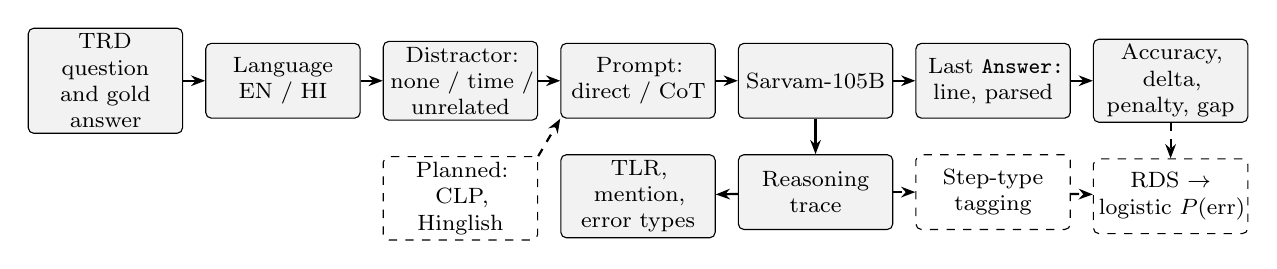
\begin{tikzpicture}[
  box/.style={draw, rounded corners=2pt, align=center, font=\footnotesize,
              minimum height=0.95cm, text width=1.82cm, inner sep=2pt, fill=gray!10},
  plan/.style={box, dashed, fill=white},
  arr/.style={-{Stealth[length=1.8mm]}, thick},
  node distance=0.45cm and 0.28cm]
\node[box] (trd) {TRD question\\and gold answer};
\node[box, right=of trd] (lang) {Language\\EN / HI};
\node[box, right=of lang] (dist) {Distractor:\\none / time /\\unrelated};
\node[box, right=of dist] (prompt) {Prompt:\\direct / CoT};
\node[box, right=of prompt] (model) {Sarvam-105B};
\node[box, right=of model] (ext) {Last \texttt{Answer:}\\line, parsed};
\node[box, right=of ext] (acc) {Accuracy, delta,\\penalty, gap};
\node[plan, below=of dist] (planprompt) {Planned: CLP,\\Hinglish};
\node[box, below=of prompt] (tlr) {TLR, mention,\\error types};
\node[box, below=of model] (trace) {Reasoning\\trace};
\node[plan, below=of ext] (tag) {Step-type\\tagging};
\node[plan, below=of acc] (rds) {RDS $\rightarrow$\\logistic $P(\mathrm{err})$};
\draw[arr] (trd) -- (lang);
\draw[arr] (lang) -- (dist);
\draw[arr] (dist) -- (prompt);
\draw[arr] (prompt) -- (model);
\draw[arr] (model) -- (ext);
\draw[arr] (ext) -- (acc);
\draw[arr] (model) -- (trace);
\draw[arr] (trace) -- (tlr);
\draw[arr, dashed] (planprompt.north east) -- (prompt.south west);
\draw[arr, dashed] (trace) -- (tag);
\draw[arr, dashed] (tag) -- (rds);
\draw[arr, dashed] (acc) -- (rds);
\end{tikzpicture}
\caption{Our pipeline. Each TRD question is posed in English or Hindi, given a distractor, and wrapped in a direct or CoT prompt before Sarvam-105B answers it; the answer is scored and the trace analysed. Solid boxes are implemented and used in this report; dashed boxes are planned.}
\label{fig:pipeline}
\end{figure*}

\section{Experimental Setup}
\label{sec:setup}

\paragraph{Data.}
Figure~\ref{fig:pipeline} shows the pipeline. TRD has nine task types: date addition and subtraction, time addition and subtraction, date and time duration, date recurrence, interval date and day of week, which its authors group into three reasoning tasks (arithmetic, duration, recurrence) and two memorisation tasks (intervals, day of week). Five difficulty levels scale the offsets and spans involved, from \emph{short} to \emph{very very long}, and each question fills a carrier phrase written with native speakers, such as ``Today is [DATE], what is the date going to be in [N] days?'' \citep{mazzia-etal-2026-benchmarking}. We extend the TRD generator so that, for each task and level, it draws 150 questions (seed 9), each with a no-distractor, a time-related and an unrelated version taken from TRD's templates, and replays the same random draws for English and Hindi. The two languages therefore share dates, offsets, gold answers and distractor choice, and differ only in wording.

\paragraph{Prompts and model.}
Both prompts share one template. The direct prompt says ``Answer the following question directly. Do not provide any reasoning or explanation. Give only the final answer.'' The CoT prompt says ``Solve the following question by reasoning through it step by step. Your reasoning must be written entirely in [language]; do not switch to another language at any point.'' Both then ask for the whole response in the question's language and for a final line of the form \texttt{Answer: <answer>} in a task-specific format, with the word \texttt{Answer:} kept in English and Western digits. We call \texttt{sarvam-105b}, a mixture-of-experts model built mainly for Indian languages, through Sarvam's API with greedy decoding (temperature 0, as in TRD), a 4,096-token output limit and the model's separate thinking mode turned off in both conditions, so that a direct answer really is direct and the CoT is the visible response.

\paragraph{Scoring and trace measures.}
We take the last \texttt{Answer:} line of a response, remove stray markdown and punctuation, convert Devanagari and Arabic-Indic digits to Western digits, and compare it with the gold answer by exact match, as TRD does; for day of week we compare the weekday itself, so that a Hindi or English spelling of the correct day both count. We measure language drift with the target-language ratio,
\begin{equation}
\mathrm{TLR}(t)=\frac{N_{\mathrm{hi}}(t)}{N_{\mathrm{hi}}(t)+N_{\mathrm{en}}(t)},
\end{equation}
where $N_{\mathrm{hi}}$ and $N_{\mathrm{en}}$ count the Devanagari and Latin-script words in trace $t$ outside the answer line; punctuation, symbols and digits count towards neither. For English traces the numerator counts English words instead. For Hinglish, where Hindi words are also written in Roman script, we will switch to word-level language identification.

\section{Progress So Far}
\label{sec:progress}

\begin{table}[t]
\centering
\small
\setlength{\tabcolsep}{3.5pt}
\begin{tabular}{@{}lrrrrr@{}}
\toprule
Task & Short & Med. & Long & V.\ long & V.V.\ long \\
\midrule
Date addition & 150 & 150 & 150 & 150 & -- \\
Date subtraction & 150 & 150 & -- & 150 & -- \\
Date duration & 150 & 150 & 135 & 150 & -- \\
Date recurrence & 150 & 150 & -- & 150 & -- \\
Day of week & 146 & 149 & -- & 150 & -- \\
Interval date & -- & -- & -- & 150 & -- \\
Time addition & -- & -- & -- & 149 & -- \\
Time subtraction & -- & -- & -- & 111 & -- \\
Time duration & -- & -- & -- & 149 & -- \\
\midrule
Total & 746 & 749 & 285 & 1309 & -- \\
\bottomrule
\end{tabular}
\caption{Questions answered in all 12 conditions, by task and difficulty level, out of 150 generated per cell. Cells marked -- were not run, or only partly run, before the API credit ran out and are left out of the analysis.}
\label{tab:coverage}
\end{table}


\paragraph{Pipeline.}
The solid boxes in Figure~\ref{fig:pipeline} are built and in use: the extended generator; an asynchronous runner that calls the Sarvam API in parallel, retries rate-limit and server errors with exponential back-off, and resumes an interrupted run without repeating finished requests; a scoring module for answer extraction, accuracy and the TLR; and analysis scripts for the measures and tests of Section~\ref{sec:analysis}. Every run is stored with a copy of its code, configuration and outputs.

\paragraph{Runs.}
Of the \NPlannedQuestions{} questions planned (nine tasks, five difficulty levels, 150 questions each), \NQuestions{} (\CoveragePct{}\%) have been answered in all 12 conditions (Table~\ref{tab:coverage}). The runs stopped when the API credit ran out, so the very-very-long level has not been run and some tasks are missing at the short, medium and long levels. We analyse only questions with all 12 responses, which keeps every comparison paired.

\paragraph{Data checks.}
We checked that the English and Hindi versions are parallel. For all \NQuestions{} questions the gold answer is identical across languages and all 12 records, the question numbers match across languages, the direct and CoT prompts share the same question, and every English distractor maps to exactly one Hindi distractor and back (35 time-related and 43 unrelated pairs).

\section{Analysis}
\label{sec:analysis}

We analyse the \NRecords{} responses to the \NQuestions{} questions answered in all 12 conditions (Section~\ref{sec:progress}). All differences are in percentage points. We can grade a response only if it ends with the requested \texttt{Answer:} line. \NCutoff{} responses (\NCutoffPct{}\%) have no such line because they reached the 4,096-token output limit and were cut off mid-reasoning; \NCutoffEnCot{} of them are English CoT. We leave these out of accuracy rather than count them as wrong, and check in Section~\ref{sec:cot-delta} that counting them as wrong changes no conclusion.

Differences between paired conditions are tested with the exact McNemar test \citep{mcnemar-1947-note} with Holm correction \citep{holm-1979-simple}, and confidence intervals (CIs) come from a 2,000-sample bootstrap that resamples questions, so that the 12 responses to a question stay together \citep{berg-kirkpatrick-etal-2012-empirical,dror-etal-2018-hitchhikers}. Square brackets give 95\% CIs, the range of values consistent with the data; an interval that excludes zero means the difference is unlikely to be due to chance.

\subsection{Does CoT help, and in which language?}
\label{sec:cot-delta}

\begin{table*}[t]
\centering
\begin{tabular}{lrrrrrrr}
\toprule
 & & \multicolumn{3}{c}{English} & \multicolumn{3}{c}{Hindi} \\
\cmidrule(lr){3-5}\cmidrule(lr){6-8}
Task & $Q$ & Direct & CoT & $\Delta$ & Direct & CoT & $\Delta$ \\
\midrule
Date addition & 600 & 93.7 & 98.5 & +4.8$^{*}$ & 89.5 & 88.3 & $-$1.2\phantom{$^{*}$} \\
Date subtraction & 450 & 93.6 & 95.9 & +2.3$^{*}$ & 92.2 & 78.2 & \textbf{$-$14.0$^{*}$} \\
Date duration & 585 & 88.9 & 99.1 & +10.2$^{*}$ & 85.1 & 87.5 & +2.5\phantom{$^{*}$} \\
Date recurrence & 450 & 24.5 & 92.4 & +67.9$^{*}$ & 4.8 & 26.0 & +21.2$^{*}$ \\
Day of week & 445 & 14.1 & 70.5 & +56.4$^{*}$ & 15.7 & 21.8 & +6.1$^{*}$ \\
Interval date & 150 & 29.8 & 43.1 & +13.3$^{*}$ & 35.1 & 17.9 & \textbf{$-$17.2$^{*}$} \\
Time addition & 149 & 57.7 & 97.1 & +39.3$^{*}$ & 60.2 & 73.5 & +13.4$^{*}$ \\
Time subtraction & 111 & 48.9 & 98.5 & +49.5$^{*}$ & 51.7 & 74.2 & +22.5$^{*}$ \\
Time duration & 149 & 58.8 & 99.8 & +40.9$^{*}$ & 28.9 & 72.6 & +43.8$^{*}$ \\
\midrule
All tasks & 3,089 & 63.2 & 91.1 & +27.9$^{*}$ & 57.7 & 62.9 & +5.1$^{*}$ \\
\bottomrule
\end{tabular}
\caption{Accuracy (\%) with direct answers and chain-of-thought (CoT), pooled over difficulty levels and distractor conditions. $Q$ is the number of questions; each question contributes three responses per language and condition. $\Delta$ is CoT minus direct in percentage points; $^{*}$ marks $p<0.05$ in an exact McNemar test on paired responses, Holm-corrected over the 18 task--language tests (uncorrected for the pooled row). Significant negative deltas are in bold. Chance for day of week is 14.3\%.}
\label{tab:cot-delta}
\end{table*}


Table~\ref{tab:cot-delta} shows the central result. CoT raises English accuracy from \EnDirectAcc{}\% to \EnCotAcc{}\% (\EnCotDelta{} points [\EnCotDeltaLo{}, \EnCotDeltaHi{}]) but Hindi accuracy only from \HiDirectAcc{}\% to \HiCotAcc{}\% (\HiCotDelta{} [\HiCotDeltaLo{}, \HiCotDeltaHi{}]). The English gain is significant in all \NEnSigPos{} tasks. In Hindi, CoT helps significantly in \NHiSigPos{} tasks and \emph{hurts} significantly in two: date subtraction (\HiSubtractionDirect{}\% $\rightarrow$ \HiSubtractionCot{}\%) and interval date (\HiIntervalDirect{}\% $\rightarrow$ \HiIntervalCot{}\%). Asking the model to reason step by step in Hindi can therefore be worse than asking it for the answer alone, and this happens without any distractor, since the table pools all three distractor conditions. The only task where Hindi gains at least as much as English is time duration (\HiTimeDurationDelta{} vs.\ \EnTimeDurationDelta{} points), where Hindi direct answers are unusually poor (\HiTimeDurationDirect{}\%).

These conclusions do not depend on how the cut-off responses are treated. Counting them as wrong, which penalises English CoT most, the CoT gain is still \EnStrictDelta{} points in English and \HiStrictDelta{} in Hindi.

\paragraph{Direct answers on two tasks are at chance.}
\input{figures/day_of_week_float}
Without CoT, day-of-week accuracy is \EnDowDirect{}\% in English and \HiDowDirect{}\% in Hindi, against a chance level of 14.3\%. Figure~\ref{fig:dow} shows that this is not a near miss. The difference between the predicted and the correct weekday is spread evenly over all seven values (\EnDowDirectMin{}--\HiDowDirectMax{}\% each), so the direct answer carries no information about the date. Instead, direct answers favour one weekday regardless of the question: \EnDowModeDay{} for \EnDowModeShare{}\% of English answers and \HiDowModeDay{} for \HiDowModeShare{}\% of Hindi answers, while the correct answers are spread roughly evenly over the week. English CoT fixes most of this (\EnDowCot{}\%), with remaining errors skewed late (+1 day: \EnDowCotPlusOne{}\%; $-$1 day: \EnDowCotMinusOne{}\%). Hindi CoT is more often exactly one day late (\HiDowCotPlusOne{}\%) than correct (\HiDowCotZero{}\%).

Date recurrence shows a similar split. In both languages, \EnRecDirectFirstStep{}\% of direct answers are ``today plus one interval'', which ignores which occurrence the question asks for. English CoT almost eliminates this shortcut (\EnRecCotFirstStep{}\%), while Hindi CoT keeps it in \HiRecCotFirstStep{}\% of answers. Hindi also produces a date in the past, today minus the interval times the occurrence number, in \HiRecDirectMirror{}\% (direct) and \HiRecCotMirror{}\% (CoT) of answers, against \EnRecDirectMirror{}\% and \EnRecCotMirror{}\% in English. The Hindi template phrases the question as \foreignlanguage{hindi}{आज को छोड़कर, 1वीं आवृत्ति की तिथि क्या है?} \emph{\={a}j ko cho\d{r}kar, 1v\={\i}\d{m} \={a}v\d{r}tti k\={\i} tithi ky\={a} hai?} (`excluding today, what is the date of the 1th occurrence?'), with a templated ordinal suffix that is non-standard for small numbers. We have not yet tested whether this wording causes the reversal; it is a possible confound in TRD's Hindi recurrence questions rather than in the model's arithmetic.

\subsection{The English--Hindi gap across difficulty}
\label{sec:difficulty}

\input{figures/difficulty_float}

We call English accuracy minus Hindi accuracy the \emph{English--Hindi gap}; a positive gap means English is ahead. Because each difficulty level contains a different mix of tasks, Figure~\ref{fig:difficulty} compares levels using only tasks present at all of them. From the short to the very long level, the gap grows far more with CoT than with direct answers. For date addition and duration it grows from \GapADirectShort{} to \GapADirectVeryLong{} points with direct answers but from \GapACotShort{} to \GapACotVeryLong{} points with CoT. Over the five date tasks, the CoT gap grows from \GapCotShort{} to \GapCotVeryLong{} points, while the direct gap stays below 9 points. On the easiest questions, Hindi CoT does not even beat Hindi direct answers (\AHiCotShort{}\% vs.\ \AHiDirectShort{}\%). The language gap is therefore mainly a gap in how much CoT helps.

\subsection{CoT under distraction}
\label{sec:distraction}

\begin{table}[t]
\centering
\small
\setlength{\tabcolsep}{4pt}
\begin{tabular}{lrrrrr}
\toprule
 & \multicolumn{3}{c}{Accuracy} & \multicolumn{2}{c}{Drop} \\
\cmidrule(lr){2-4}\cmidrule(lr){5-6}
 & None & Sim. & Dis. & Sim. & Dis. \\
\midrule
\multicolumn{6}{l}{\textit{English}} \\
\quad Direct & 63.9 & 63.0 & 62.7 & +0.9 & +1.2 \\
\quad CoT & 91.6 & 90.6 & 91.2 & +0.9 & +0.4 \\
\quad CoT $-$ direct &  &  &  & +0.0 & $-$0.8 \\
\midrule
\multicolumn{6}{l}{\textit{Hindi}} \\
\quad Direct & 57.4 & 58.1 & 57.7 & $-$0.7 & $-$0.3 \\
\quad CoT & 65.2 & 60.7 & 62.7 & +4.5 & +2.5 \\
\quad CoT $-$ direct &  &  &  & \textbf{+5.2} & \textbf{+2.8} \\
\bottomrule
\end{tabular}
\caption{Accuracy (\%) with no distractor (None), a time-related (Sim.) or an unrelated (Dis.) distractor. Drop is accuracy without the distractor minus accuracy with it (points; positive means the distractor hurt). CoT $-$ direct is the CoT drop minus the direct drop (the CoT distraction penalty); bold marks a 95\% cluster-bootstrap interval that excludes zero.}
\label{tab:distractor}
\end{table}


Our main hypothesis was that CoT gives a distractor more opportunities to enter the reasoning and change the answer. Table~\ref{tab:distractor} supports this only in Hindi. In English, neither distractor lowers accuracy by more than \EnMaxDrop{} points under either prompting condition. In Hindi, direct answers are unaffected by the similar distractor (accuracy changes by \HiDropDirectSim{} points), but CoT accuracy falls by \HiDropCotSimAbs{} points. CoT therefore loses \HiDidSimAbs{} more points to the distractor than direct answering does [\HiDidSimLo{}, \HiDidSimHi{}]; we call this extra loss the \emph{CoT distraction penalty} (the ``CoT $-$ direct'' row of Table~\ref{tab:distractor}). In English the penalty is \EnDidSim{} [\EnDidSimLo{}, \EnDidSimHi{}]. The unrelated distractor also carries a smaller penalty in Hindi (\HiDidDis{} [\HiDidDisLo{}, \HiDidDisHi{}]). Computing the Hindi penalty for the similar distractor separately for each task shows that it comes mostly from date duration (\HiDidSimDuration{} points [\HiDidSimDurationLo{}, \HiDidSimDurationHi{}]), day of week (\HiDidSimDow{} [\HiDidSimDowLo{}, \HiDidSimDowHi{}]) and time duration (\HiDidSimTimeDuration{} [\HiDidSimTimeDurationLo{}, \HiDidSimTimeDurationHi{}]). Previous work found that irrelevant context distracts models on arithmetic word problems \citep{shi-etal-2023-distracted}; here the susceptibility is specific to one language and to the reasoning condition.

\paragraph{Does the distractor enter the trace?}
We count a trace as mentioning the distractor if it contains a content word of the distractor that does not occur in the question (function words and generic time words such as ``day'' are excluded). Some of these words can appear in a trace by coincidence, for example month names in a trace about dates. To measure this chance rate we use a \emph{placebo}: for each question we take the trace written without any distractor and search it for the words of the distractor that would have been inserted. The model never saw those words, so any match there is coincidence. The difference between the two rates is the share of traces that really take up the distractor. Hindi traces take up the distractor far more often than English ones (Table~\ref{tab:trace}): \HiMentionDis{}\% of Hindi traces mention the unrelated distractor (placebo \HiMentionDisPlacebo{}\%), against \EnMentionDis{}\% in English (placebo \EnMentionDisPlacebo{}\%). Hindi traces often build the distractor into the narrative of the solution. For the short date-addition question that starts ``The garden needs new flowers'', a correct Hindi trace ends with
\begin{quote}
\foreignlanguage{hindi}{इस तरह, बगीचे में नए फूल लगाने के लिए सही तारीख 2025-03-30 है।}\\
\emph{is tarah, bag\={\i}ce me\d{m} nae ph\={u}l lag\={a}ne ke lie sah\={\i} t\={a}r\={\i}kh 2025-03-30 hai.}\\
`Thus, the correct date for planting new flowers in the garden is 2025-03-30.'
\end{quote}
Appendix~\ref{app:mention} relates these mentions to answer correctness. The distractor also leaks into wrong answers. For example, after the distractor ``February is such a unique month with its varying days'', a Hindi direct answer to a recurrence question whose correct answer is \mbox{2025-04-10} was \mbox{2025-02-06}. Overall, \HiReuseDirect{}\% (\HiReuseDirectN{}) of wrong Hindi direct answers contain a number, month or weekday taken from the similar distractor. With the same placebo as above (wrong answers to the same questions asked without the distractor, checked against the distractor that would have been inserted), this happens in only \HiReuseDirectPlacebo{}\% (\HiReuseDirectPlaceboN{}), so the difference is not chance (Fisher's exact test, \HiReuseDirectP{}). In English the two rates do not differ (\EnReuseDirect{}\% vs.\ \EnReuseDirectPlacebo{}\%, \EnReuseDirectP{}). In Hindi direct answers, the distractor therefore changes what the wrong answers are without changing how many there are.

\subsection{Properties of the reasoning traces}
\label{sec:traces}

\begin{table}[t]
\centering
\small
\setlength{\tabcolsep}{4pt}
\begin{tabular}{lrr}
\toprule
 & English & Hindi \\
\midrule
Cut off before answering & 3.0\% & 0.7\% \\
Median length (words) & 103 & 79 \\
Median completion tokens & 327 & 198 \\
Target-language ratio & 1.000 & 0.986 \\
Ratio below 0.9 & 0.0\% & 2.4\% \\
Has a verification step & 79.1\% & 1.5\% \\
Answer value in trace & 99.9\% & 99.0\% \\
Mentions sim.\ distractor & 15.1\% (10.4) & 31.8\% (8.3) \\
Mentions dis.\ distractor & 18.7\% (8.5) & 35.9\% (1.4) \\
\bottomrule
\end{tabular}
\caption{Properties of CoT responses. All rows except the first are computed over graded responses. The target-language ratio is the number of target-language words divided by the number of Hindi plus English words, with both counts summed over all responses before dividing, so longer traces weigh more. Distractor mention rates are for traces whose prompt contained that distractor; the value in parentheses is the placebo rate for the same questions without it.}
\label{tab:trace}
\end{table}


\paragraph{The model stays in Hindi, and drifting into English helps.}
The target-language ratio (Table~\ref{tab:trace}), the share of a trace's words that are in Hindi, is \HiRatioPooled{} for Hindi traces, and only \HiRatioBelow{}\% of them contain more than 10\% English words (ratio below 0.9). We call these \emph{drifting} traces. The Hindi results above therefore reflect reasoning written in Hindi. The \HiNRatioBelow{} drifting traces look less accurate overall (\HiAccRatioBelow{}\% vs.\ \HiAccRatioAbove{}\%), but mainly because of which questions they occur on: \DriftDow{} of them are day-of-week questions, one of the two hardest tasks for Hindi CoT. Compared within the same task, drifting traces are more accurate: \DriftDowAcc{}\% vs.\ \DriftDowAccNo{}\% on day of week and \DriftRecAcc{}\% vs.\ \DriftRecAccNo{}\% on date recurrence. Combining all tasks this way, a drifting trace has about twice the odds of a correct answer (Appendix~\ref{app:drift}). This agrees with the finding that English intermediate steps can match or beat steps in the question's language \citep{shi-etal-2023-mgsm}, and it motivates the cross-lingual prompting condition \citep{qin-etal-2023-cross} that we run next.

\paragraph{Hindi traces are shorter and rarely check their work.}
Hindi traces are shorter than English ones (median \HiMedianWords{} vs.\ \EnMedianWords{} words; \HiMedianTokens{} vs.\ \EnMedianTokens{} completion tokens). \EnVerification{}\% of English traces contain a verification step (``let me verify'', ``alternatively''), against \HiVerification{}\% of Hindi traces. Verification does not explain the English advantage, however. English traces with a verification step look less accurate overall (\VerAccWith{}\% vs.\ \VerAccWithout{}\%), but again because verification is most common in the hardest tasks; compared within the same task, verifying makes no clear difference to accuracy (Appendix~\ref{app:verification}).

\paragraph{Answers follow the trace.}
The final answer value appears in the trace in \EnAnswerInTrace{}\% of English and \HiAnswerInTrace{}\% of Hindi CoT responses, and only \EnWrongEndsGold{} of \EnWrong{} wrong English answers and \HiWrongEndsGold{} of \HiWrong{} wrong Hindi answers come from a trace whose last value was the correct one. Wrong answers are therefore wrong in the trace, not copied wrongly at the end. This is consistency between trace and answer, not evidence that the trace reflects the model's internal computation \citep{turpin-etal-2023-unfaithful}.

\subsection{Language-specific failures and error types}
\label{sec:errors}

Every question was asked in both languages, so we can pair the English and Hindi responses to the same question, distractor and prompting condition and ask whether the two languages fail on the same questions. Under CoT, of \AgreeCotPairs{} pairs, both are right in \AgreeCotBothRight{} and both wrong in \AgreeCotBothWrong{}; when they disagree, English is almost always the one that is right (\AgreeCotEnOnly{} pairs, against \AgreeCotHiOnly{} where only Hindi is right). If Hindi failed mainly on questions that are hard in any language, the two languages would tend to fail together. We measure this with the $\phi$ coefficient, a correlation between two right/wrong outcomes (0: unrelated, 1: always the same), computed within each task and difficulty so that differences between tasks do not inflate it. With direct answers the median $\phi$ is \AgreeDirectPhi{}: the languages partly fail on the same, harder questions. With CoT it is \AgreeCotPhi{}: whether Hindi CoT is right has almost nothing to do with whether English CoT is right on the same question. Hindi CoT failures are therefore specific to Hindi rather than a sign of hard questions.

The errors also differ in kind (Figure~\ref{fig:errors} in Appendix~\ref{app:errors}). \EnErrAllOffByOne{}\% of wrong English CoT answers are off by one day (\EnErrAddOffByOne{}\% in date addition and \EnErrSubOffByOne{}\% in date subtraction), the slip of an otherwise correct procedure. Only \HiErrAllOffByOne{}\% of wrong Hindi CoT answers are off by one. The rest include month slips, where the day and year are right but the month is wrong (\HiErrAddMonthSlip{}\% of Hindi date-addition errors, none in English), and the reversed direction in date recurrence discussed in Section~\ref{sec:cot-delta}. Hindi CoT does not just make more of the same mistakes as English CoT; it often follows a different, wrong procedure.


\section{Timeline and Remaining Work}
\label{sec:timeline}

\begin{table}[t]
\centering
\small
\setlength{\tabcolsep}{4pt}
\begin{tabular}{@{}lp{5.6cm}@{}}
\toprule
Week & Work \\
\midrule
5--11 Oct & Top up API credit; finish the missing short, medium and long runs (Table~\ref{tab:coverage}) and run the very-very-long level. \\
\addlinespace[5pt]
12--18 Oct & Hinglish reasoning condition and word-level language identification for its TLR; rerun Hindi date recurrence with a reworded question to test the template confound; start the rule-based step-type tagger. \\
\addlinespace[5pt]
19--25 Oct & CLP for Hindi questions, and CLSP with English and Hindi if time allows, compared with Hindi CoT; finish the step-type tagger and hand-tag a sample of traces to validate it and the mention, reuse and verification heuristics. \\
\addlinespace[5pt]
26--31 Oct & RDS and the logistic model $P(\mathrm{err})$ from RDS, difficulty and language; significance tests across all conditions; final analysis, report and viva preparation. \\
\bottomrule
\end{tabular}
\caption{Timeline for the rest of the project (deadline 31 October).}
\label{tab:timeline}
\end{table}

Table~\ref{tab:timeline} lists the remaining work. Completing the grid comes first; the new conditions follow in order of dependence, since Hinglish needs only a new instruction, CLP a second turn, and RDS a tagger validated by hand. 

\section{Conclusion}
\label{sec:conclusion}

On \NQuestions{} TRD questions answered in English and Hindi, with and without distractors, CoT helps Sarvam-105B far more in English than in Hindi, the gap grows with difficulty, and distractors harm CoT only in Hindi, where they often become part of the reasoning. The remaining work tests whether Hinglish reasoning or an English restatement closes this gap, and whether Hindi traces that diverge from English ones fail more.

\section*{Limitations}

All results come from one model, decoded greedily with one prompt template, so they describe this configuration rather than CoT in general. Our runs stopped early when the API credit ran out, so the data cover only four of the five TRD difficulty levels and not every task at every level; Figure~\ref{fig:difficulty} works around this by comparing levels only on tasks present at all of them. Three of our measures, whether a trace mentions the distractor, whether a wrong answer reuses it, and whether a trace verifies its work, are simple word-matching rules rather than human judgements. They can miss a paraphrased mention and can count a word that appears for an unrelated reason. The placebo rates estimate how often such accidental matches happen, and comparing within each task removes differences between tasks, but neither catches missed paraphrases; we will check a hand-labelled sample for the final report. Cut-off responses are excluded from accuracy and are concentrated in English CoT, but counting them as wrong changes no conclusion. Finally, the CLP, Hinglish and trace-structure conditions are not yet run, so the claims here are limited to direct answers and CoT in the question's own language.

\bibliography{references}

\clearpage
\appendix
\section{Odds-Ratio Analyses of CoT Traces}
\label{app:or}

We relate three properties of CoT traces to answer correctness: mentioning the distractor, drifting into English, and containing a verification step. Pooled comparisons are misleading here, because tasks differ in both accuracy and how often each property occurs, and pooled comparisons can reverse \citep{simpson-1951-interpretation}; this happens for drift and for verification. We therefore compare traces with and without the property within each task and difficulty, and combine these groups with a Mantel--Haenszel odds ratio (OR) \citep{mantel-haenszel-1959-statistical}, using only groups that contain traces of both kinds. An OR of 1 means no difference; an OR above 1 means that traces with the property are more often correct, and an OR below 1 that they are less often correct. Square brackets give 95\% CIs.

\subsection{Distractor Mentions}
\label{app:mention}

\begin{table}[ht]
\centering
\small
\begin{tabular}{llrr}
\toprule
Distractor & Language & Traces & OR [95\% CI] \\
\midrule
Time-related & English & 2,974 & 0.64 [0.44, 0.93] \\
 & Hindi & 3,066 & 0.77 [0.63, 0.95] \\
\midrule
Unrelated & English & 3,015 & 1.33 [0.82, 2.15] \\
 & Hindi & 3,073 & 1.11 [0.90, 1.36] \\
\bottomrule
\end{tabular}
\caption{Odds ratio (OR) of a correct answer for CoT traces that mention the distractor versus traces that do not, stratified by task and difficulty (Mantel--Haenszel). Traces is the number of CoT responses whose prompt contained that distractor.}
\label{tab:mention-or}
\end{table}


Table~\ref{tab:mention-or} compares CoT traces that mention the distractor (Section~\ref{sec:distraction}) with traces that do not. Traces that mention the time-related distractor have about \EnMentionSimOddsDrop{}\% (English) and \HiMentionSimOddsDrop{}\% (Hindi) lower odds of a correct answer, and both intervals lie below 1. For the unrelated distractor both intervals include 1, so mentioning it is not linked to accuracy: the model brings it up and then ignores it.

\subsection{Language Drift}
\label{app:drift}

Section~\ref{sec:traces} compares drifting Hindi CoT traces (target-language ratio below 0.9) with the other Hindi CoT traces. Drifting traces are concentrated in the hardest tasks, so they look less accurate when pooled. Within task and difficulty, over the \DriftStrata{} groups that contain both kinds of trace, the OR is \DriftOR{} [\DriftORLo{}, \DriftORHi{}] (\DriftP{}): a drifting trace has about twice the odds of a correct answer. This comparison is observational; drifting may accompany easier instances within a task rather than cause correct answers, which the cross-lingual prompting condition will test directly.

\subsection{Verification Steps}
\label{app:verification}

English traces with a verification step look less accurate when pooled (\VerAccWith{}\% vs.\ \VerAccWithout{}\%), but verification is concentrated in the hardest tasks: it appears in \VerDowN{} of the \VerDowTotal{} graded English day-of-week traces. Within task and difficulty, the OR is \VerOR{} [\VerORLo{}, \VerORHi{}] (\VerP{}). The interval includes 1, so verifying makes no clear difference to accuracy, and the much higher rate of verification in English (\EnVerification{}\% vs.\ \HiVerification{}\%) does not explain the English advantage.

\section{Error Types}
\label{app:errors}

\input{figures/error_types_float}


\end{document}
